\documentclass[12pt]{article}

\title{Activity 11: Objects}
\author{Dr. Chris Mayfield}
\date{CS 149, Fall 2016}

%\ProvidesPackage{cspogil}

% fonts
\usepackage[utf8]{inputenc}
\usepackage[T1]{fontenc}
\usepackage{mathpazo}

% spacing
\usepackage[margin=2cm]{geometry}
\renewcommand{\arraystretch}{1.4}
\setlength{\parindent}{0pt}

% orphans and widows
\clubpenalty=10000
\widowpenalty=10000
\pagestyle{empty}

% figures and tables
\usepackage{graphicx}
\usepackage{multicol}
\usepackage{tabularx}
\usepackage{wrapfig}

% fixed-width columns
\usepackage{array}
\newcolumntype{L}[1]{>{\raggedright\let\newline\\\arraybackslash\hspace{0pt}}m{#1}}
\newcolumntype{C}[1]{>{\centering\let\newline\\\arraybackslash\hspace{0pt}}m{#1}}
\newcolumntype{R}[1]{>{\raggedleft\let\newline\\\arraybackslash\hspace{0pt}}m{#1}}

% include paths
\makeatletter
\def\input@path{{Models/}{../../Models/}}
\graphicspath{{Models/}{../../Models/}}
\makeatother

% colors
\usepackage[svgnames,table]{xcolor}
\definecolor{bgcolor}{HTML}{FAFAFA}
\definecolor{comment}{HTML}{007C00}
\definecolor{keyword}{HTML}{0000FF}
\definecolor{strings}{HTML}{B20000}

% table headers
\newcommand{\tr}{\bf\cellcolor{Yellow!10}}

% syntax highlighting
\usepackage{textcomp}
\usepackage{listings}
\lstset{
    basicstyle=\ttfamily\color{black},
    backgroundcolor=\color{bgcolor},
    numberstyle=\scriptsize\color{comment},
    commentstyle=\color{comment},
    keywordstyle=\color{keyword},
    stringstyle=\color{strings},
    columns=fullflexible,
    keepspaces=true,
    showlines=true,
    showstringspaces=false,
    upquote=true
}

% code environments
\newcommand{\java}[1]{\lstinline[language=java]{#1}}%[
\lstnewenvironment{javalst}{\lstset{language=java,backgroundcolor=}}{}
\lstnewenvironment{javabox}{\lstset{language=java,frame=single,numbers=left}\quote}{\endquote}

% PDF properties
\usepackage[pdftex]{hyperref}
\urlstyle{same}
\makeatletter
\hypersetup{
  pdftitle={\@title},
  pdfauthor={\@author},
  pdfsubject={\@date},
  pdfkeywords={},
  bookmarksopen=false,
  colorlinks=true,
  citecolor=black,
  filecolor=black,
  linkcolor=black,
  urlcolor=blue
}
\makeatother

% titles
\makeatletter
\renewcommand{\maketitle}{\begin{center}\LARGE\@title\end{center}}
\makeatother

% boxes [optional height]
\newcommand{\emptybox}[1][10em]{
\vspace{1em}
\begin{tabularx}{\linewidth}{|X|}
\hline\\[#1]\hline
\end{tabularx}}

% models
\newcommand{\model}[1]{\section{#1}\nopagebreak}
\renewcommand{\thesection}{Model~\arabic{section}}

% questions
\newcommand{\quest}[1]{\subsection*{Questions~ (#1)}}
\newcounter{question}
\newcommand{\Q}{\vspace{1em}\refstepcounter{question}\arabic{question}.~ }
\renewcommand{\thequestion}{\#\arabic{question}}

% sub-question lists
\usepackage{enumitem}
\setenumerate[1]{label=\alph*)}
\setlist{itemsep=1em,after=\vspace{1ex}}

% inline answers
\definecolor{answers}{HTML}{C0C0C0}
\newcommand{\ans}[1]{%
\ifdefined\Student
    \leavevmode\phantom{~~\textcolor{answers}{#1}}
\else
    ~~\textcolor{answers}{#1}
\fi}

% longer answers [optional height]
\newsavebox{\ansbox}
\newenvironment{answer}[1][4em]{
\nopagebreak
\begin{lrbox}{\ansbox}
\begin{minipage}[t][#1]{\linewidth}
\color{answers}
}{
\end{minipage}
\end{lrbox}
\ifdefined\Student
    \phantom{\usebox{\ansbox}}%
\else
    \usebox{\ansbox}%
\fi}


\begin{document}

\maketitle

Previously we explored how classes define attributes and methods.
Static variables and methods apply to the whole class, whereas non-static variables and methods apply to specific objects.
%In this activity, we'll take a closer look at what objects look like.

% based on Model 1 of "Improved Scope" activity by Helen Hu

\model{Variable Scope}

As a team, review and discuss the \java{Circle} and \java{SwapDriver} classes found on the next page at the end of the questions.
Identify the \emph{scope} of each variable based on the table below.

\begin{center}
\small
\begin{tabular}{|L{95pt}|L{125pt}|L{115pt}|L{105pt}|}
\hline
\tr &
\tr \textbf{Where declared?} &
\tr \textbf{Where used?} &
\tr \textbf{Example} \\
\hline
\textbf{static variables} \par (``class variables'') &
declared outside of all methods (typically at the start of the class) &
anywhere in the class (or in other classes if also \java{public}) &
\java{circleCount} in the \java{Circle} class \\
\hline
\textbf{instance variables} \par (``attributes'') &
declared outside of all methods (typically after any static variables) &
any non-static method (or in static methods when another object has been created) &
\java{radius} in the \java{Circle} class \\
\hline
\textbf{parameters} &
declared inside the ()'s of a method signature &
anywhere within the method where they are declared &
\java{radius} in the \java{Circle} constructor \\
\hline
\textbf{local variables} &
declared inside a method (or inside another block of code, like a \java{for} loop) &
anywhere within the method or code block after they are declared &
\java{temp} in the \java{swapInts} method \\
\hline
\end{tabular}
\end{center}


\quest{20 min}


\Q Identify one static variable from the \java{Circle} class.
\begin{enumerate}
\item What is the name and purpose of the variable?
\\ \ans{\java{circleCount} -- tracks the number of \java{Circle} objects that have been created} \\[-2em]

\item What is the scope of the variable?
\\ \ans{{\tt private static} -- it can be used anywhere within the \java{Circle} class only} \\[-2em]

\item What is one example of somewhere it cannot be used?
\\ \ans{\tt SwapDriver.main} \\[-2em]

\end{enumerate}


\Q Identify one instance variable from the \java{Circle} class.
\begin{enumerate}
\item What is the name and purpose of the variable?
\\ \ans{\java{radius} -- stores the radius of {\tt this} circle} \\[-2em]

\item What is the scope of the variable?
\\ \ans{{\tt private} and non-{\tt static} -- it can only be used in \java{Circle} in non-static contexts} \\[-2em]

\item What is one example of somewhere it cannot be used?
\\ \ans{\tt SwapDriver.main} \\[-2em]
\end{enumerate}


\Q Identify an example of where an instance variable is used within a static method.
\begin{enumerate}
\item In which method does this occur?
\\ \ans{\java{radius} is used in the \java{swapCircles} method} \\[-2em]

\item Why is the method able to access these instance variables, even though they are private?
\\ \ans{\java{swapCircles} belongs to the \java{Circle} class} \\[-2em]

\item Explain how this method is not a violation of the rule that instance variables cannot be accessed inside a static method.
\\ \ans{You can't use {\tt this}.radius in a {\tt static} method, but it's okay to use \java{c1.radius}} \\[-2em]
\end{enumerate}


\Q Identify one parameter from the \java{Circle} class.
\begin{enumerate}
\item What is the name and purpose of the variable?
\\ \ans{Possible answers include: \java{radius} (in the constructor), \java{x} and \java{y}, \java{c1} and \java{c2}} \\[-2em]

\item What is the scope of the variable?
\\ \ans{The variable exists throughout the entire method (but not other methods).} \\[-2em]

\item Where can the variable not be used?
\\ \ans{It can't be used in other methods, e.g., you can't refer to \java{x} in \java{swapCircles}.} \\[-2em]
\end{enumerate}


\Q Identify one local variable from the \java{Circle} class.
\begin{enumerate}
\item What is the name and purpose of the variable?
\\ \ans{Possible answers include: \java{temp} and \java{r} (both used for swapping values)} \\[-2em]

\item What is the scope of the variable?
\\ \ans{The variable exists from when it's declared until the end of the method.} \\[-2em]

\item Where can the variable not be used?
\\ \ans{It cannot be used in other methods and/or before it has been declared.} \\[-2em]
\end{enumerate}

\Q In the space below, predict the output of the \java{SwapDriver} program.
Why are the results different when swapping integers and swapping Circle objects?

\begin{answer}[14em]
\begin{minipage}{190pt}

\begin{javaans}
BEFORE swap:
a = 7
b = 4
    Inside swapInts
    swapping integers 7 and 4
    finished swapping 4 and 7
AFTER swap:
a = 7
b = 4
\end{javaans}

\end{minipage}
\hspace{1em}
\begin{minipage}{290pt}

\begin{javaans}
BEFORE swap:
first = Circle(7)
second = Circle(4)
    Inside swapCircles
    swapping circles Circle(7) and Circle(4)
    finished swapping Circle(4) and Circle(7)
AFTER swap:
first = Circle(4)
second = Circle(7)
\end{javaans}

\end{minipage}
\begin{javaans}
This program created 2 circles
\end{javaans}
\end{answer}

\newpage

\begin{javabox}
public class Circle {
    
    private static int circleCount = 0;
    
    private double radius;
    
    public Circle(double radius) {
        circleCount++;
        if (radius > 0) {
            this.radius = radius;
        } else {
            this.radius = 1;
        }
    }
    
    public static int getCircleCount() {
        return circleCount;
    }
    
    public double getRadius() {
        return this.radius;
    }
    
    public static void swapInts(int x, int y) {
        System.out.println("\tInside swapInts");
        System.out.println("\tswapping integers " + x + " and " + y);
        int temp = x;
        x = y;
        y = temp;
        System.out.println("\tfinished swapping " + x + " and " + y);
    }
    
    public static void swapCircles(Circle c1, Circle c2) {
        System.out.println("\tInside swapCircles");
        System.out.println("\tswapping circles " + c1 + " and " + c2);
        double r = c1.radius;
        c1.radius = c2.radius;
        c2.radius = r;
        System.out.println("\tfinished swapping " + c1 + " and " + c2);
    }
    
    public String toString() {
        return String.format("Circle(%.0f)", this.radius);
    }
}
\end{javabox}

\newpage

\begin{javabox}
public class SwapDriver {
    
    public static void main(String[] args) {
        
        // first try swapping integers
        int a = 7, b = 4;
        System.out.println("BEFORE swap:");
        System.out.println("a = " + a);
        System.out.println("b = " + b);
        Circle.swapInts(a, b);
        System.out.println("AFTER swap:");
        System.out.println("a = " + a);
        System.out.println("b = " + b);
        System.out.println();
        
        // next try swapping Circle radii
        Circle first, second;
        first = new Circle(7);
        second = new Circle(4);
        System.out.println("BEFORE swap:");
        System.out.println("first = " + first);
        System.out.println("second = " + second);
        Circle.swapCircles(first, second);
        System.out.println("AFTER swap:");
        System.out.println("first = " + first);
        System.out.println("second = " + second);
        System.out.println();
        
        System.out.printf("This program created %d circles",
                          Circle.getCircleCount());
        System.out.println();
    }
}
\end{javabox}

\newpage

% based on Model 2 of "Activity 10 - Class Design" by Helen Hu

\model{Class Design}

Classes are often used to represent abstract data types, such as \java{Color} or \java{Point}.
They are also used to represent objects in the real world, such as \java{CreditCard} (see next page) or \java{Person}.
%UML class diagrams summarize the attributes and methods of a class.

\begin{center}
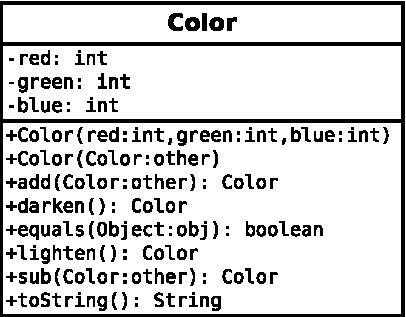
\includegraphics{Color.pdf}  % immutable
~~~~~
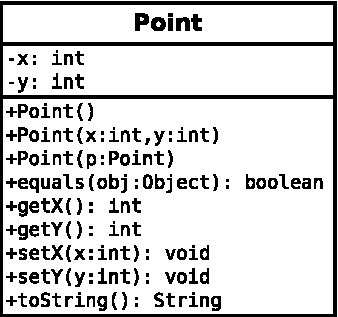
\includegraphics{Point.pdf}  % mutable
\end{center}

Classes generally include the following kinds of methods (in addition to others):
\begin{itemize}[itemsep=0pt]
\item \textbf{constructor} methods that initialize new objects
\item \textbf{accessor} methods (getters) that return attributes
\item \textbf{mutator} methods (setters) that modify attributes
\item \textbf{object} methods such as \java{equals} and \java{toString}
%\item \textbf{utility} methods which are generally static
\end{itemize}


\quest{20 min}


\Q Identify the constructors for the \java{Color} class. What is the difference between them? What arguments do they take?

\begin{answer}
There are two constructors: one that takes three integers for the RGB values, and other that takes a Color object. The latter is called a \emph{copy constructor}. Constructors do not return values.
\end{answer}


\Q Identify an accessor method in the \java{Point} class. 
\begin{enumerate}[itemsep=1pt]
\item Which instance variable does it get? \ans{{\tt this.x} or {\tt this.y}}
\item What arguments does the method take? \ans{none}
\item What does the method return? \ans{The value of \java{x} or \java{y}}
\end{enumerate}


\Q Identify a mutator method in the \java{Point} class.
\begin{enumerate}[itemsep=1pt]
\item Which instance variable does it set? \ans{{\tt this.x} or {\tt this.y}}
\item What arguments does the method take? \ans{The value of \java{x} or \java{y}}
\item What does the method return? \ans{nothing}
\end{enumerate}


\begin{center}
\textit{For the remaining questions, you will design a class that represents an individual's credit card.}
\bigskip\par
% https://www.bankofamerica.com/credit-cards/

\includegraphics{credit-card.png}
\end{center}


\Q List two or more attributes that would be necessary for this \java{CreditCard} class. For each attribute, indicate what data type would be most appropriate.

\begin{answer}[5em]
Answers may include \verb|number:long|, \verb|expire:Date|, \verb|name:String|, \verb|code:int|, etc.
\end{answer}


\Q When constructing (or updating) a \java{CreditCard} object, what values would you need to check? What are the valid ranges of values for each attribute?

\begin{answer}[5em]
The number should have 16 digits, dates need to have valid months and days, names should be at most 22 letters and not contain digits or other characters, code should be 3--4 digits.
\end{answer}


\Q List two accessor methods would be appropriate for the \java{CreditCard} class.
Include arguments and return values, using the same format as a UML diagram.

\begin{answer}[5em]
\begin{verbatim}
+getNumber(): long
+getExpire(): Date
+getName(): String
+getCode(): int
\end{verbatim}
\end{answer}


\Q List two mutator methods would be appropriate for the \java{CreditCard} class.
Include arguments and return values, using the same format as a UML diagram.

\begin{answer}[5em]
\begin{verbatim}
+setNumber(number:long): void
+setExpire(expire:Date): void
+setName(name:String): void
+setCode(code:int): void
\end{verbatim}
\end{answer}


\end{document}
